\chapter{Model Evaluation and Results Analysis}
\label{chap:Chapter4}

This chapter provides an in-depth analysis of the performance and results obtained from testing the models in two distinct environments: the local testing environment and the live testing environment.

\section{Local Testing Environment}

The models were evaluated using a dataset that was split into training and testing subsets. 
The performance of the models, specifically the RF model, was assessed using this dataset. 

Since hardware limitations prevented effective training of the RL model on this environments, only the RF model's results are presented in this section\footnote{Training a single alert takes 10 to 15 minutes, making it impractical to train on 100k alerts in a reasonable timeframe.}.

As a result, the analysis primarily highlights the RF model's performance and its evolution from Version 1 to Version 11.

The evaluation of the RF model was performed using metrics such as accuracy, precision, recall, and F1-score, all of which were computed for both priority and taxonomy predictions. 

Version 1, achieved an overall accuracy of 82\% for both priority and taxonomy predictions, with P1 and P2 classes performing relatively well. 
However, the model struggled with the minority categories, especially Abusive Content and Vulnerable taxonomy classes, as reflected in Figures~\ref{fig:confusion_priority_v1} and \ref{fig:confusion_taxonomy_v1} the confusion matrix.

As the model evolved, Version 11 showed significant improvements, particularly in the recall for minority classes. 
The final model achieved 90\% accuracy for priority classification and 92\% for taxonomy, demonstrating better handling of low-frequency categories and fewer misclassifications.

The following confusion matrices, Figures~\ref{fig:confusion_priority_v1}, \ref{fig:confusion_taxonomy_v1}, \ref{fig:confusion_priority_v11}, and \ref{fig:confusion_taxonomy_v11}, show the performance of Version 1 and Version 11, highlighting the improvement in both priority and taxonomy classifications from the first to the last version.

\clearpage 

% \begin{figure}[t!]
%     \centering
%     \begin{minipage}{0.49\textwidth}
%         \centering
%         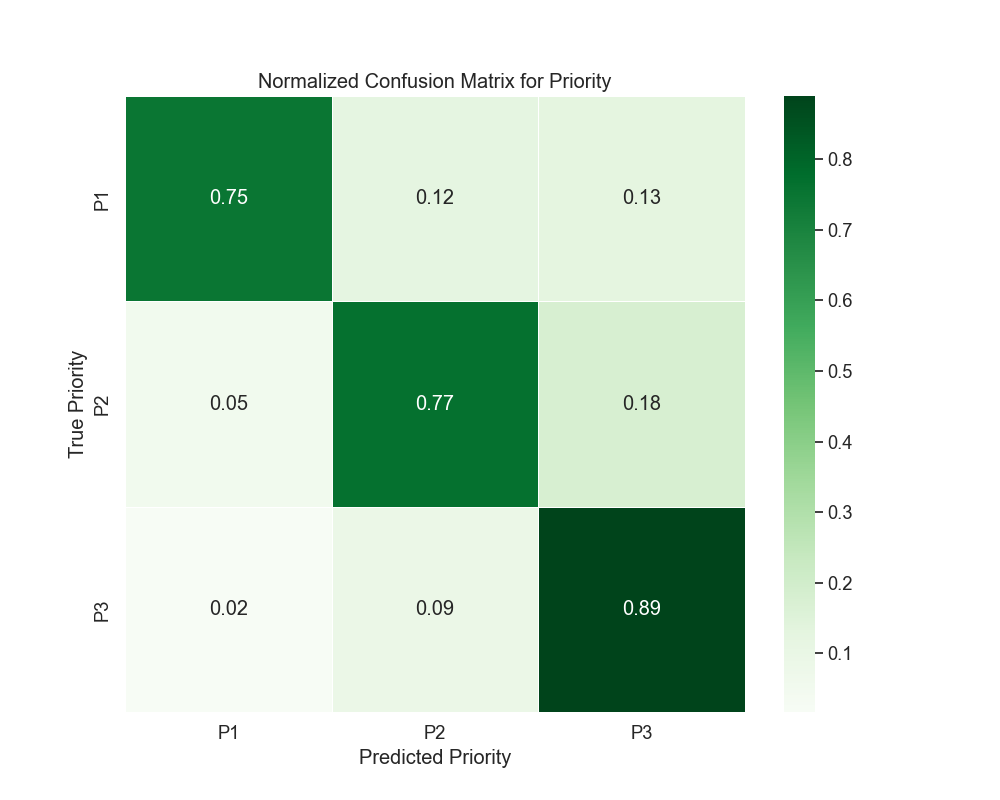
\includegraphics[width=\textwidth]{ch4/assets/v1_confusion_priority.png}
%         \caption{Confusion Matrix for Priority (Version 1)}
%         \label{fig:confusion_priority_v1}
%     \end{minipage}
%     \hfill
%     \begin{minipage}{0.49\textwidth}
%         \centering
%         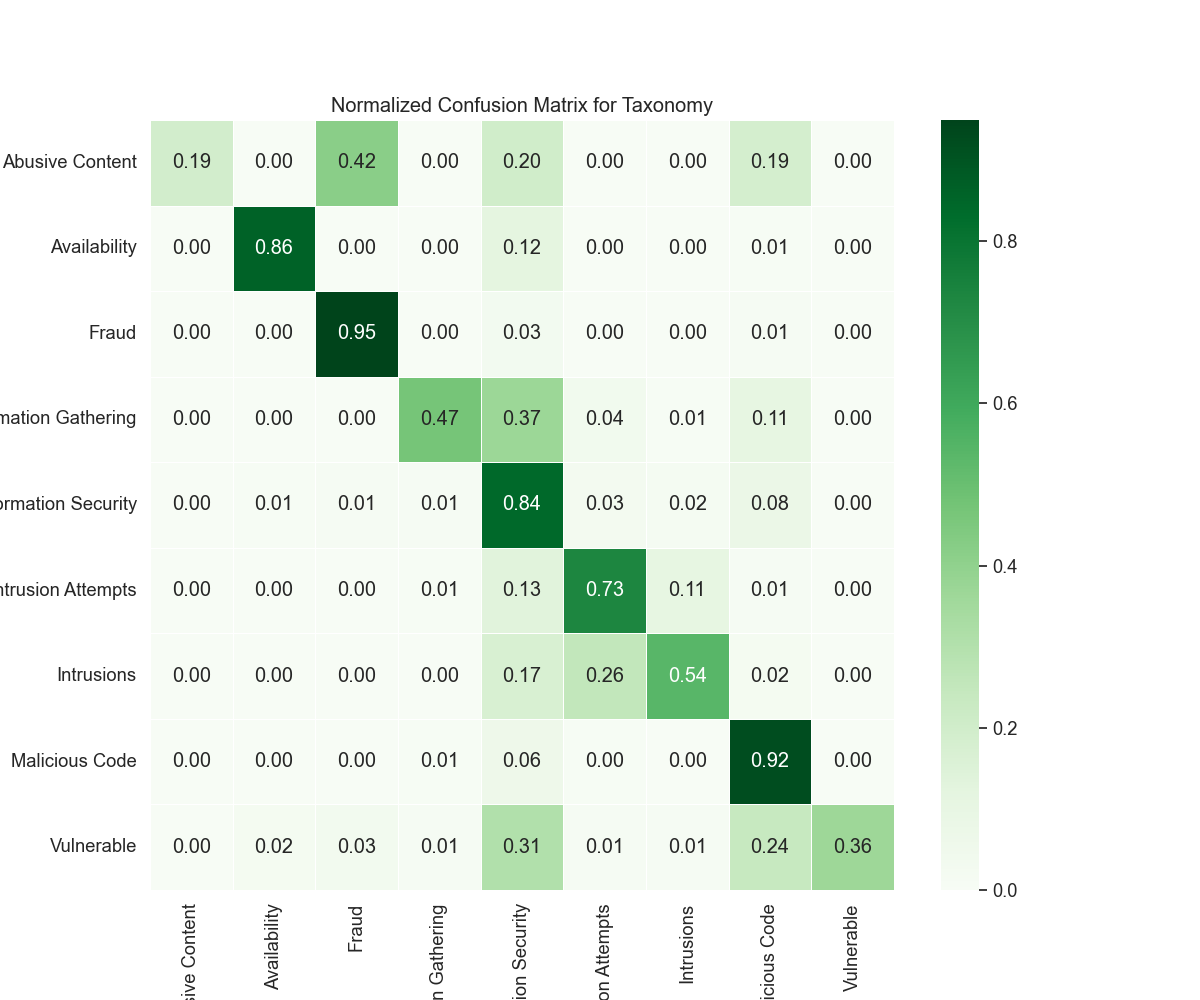
\includegraphics[width=\textwidth]{ch4/assets/v1_confusion_taxonomy.png}
%         \caption{Confusion Matrix for Taxonomy (Version 1)}
%         \label{fig:confusion_taxonomy_v1}
%     \end{minipage}
% \end{figure}

% \begin{figure}[h!]
%     \centering
%     \begin{minipage}{0.49\textwidth}
%         \centering
%         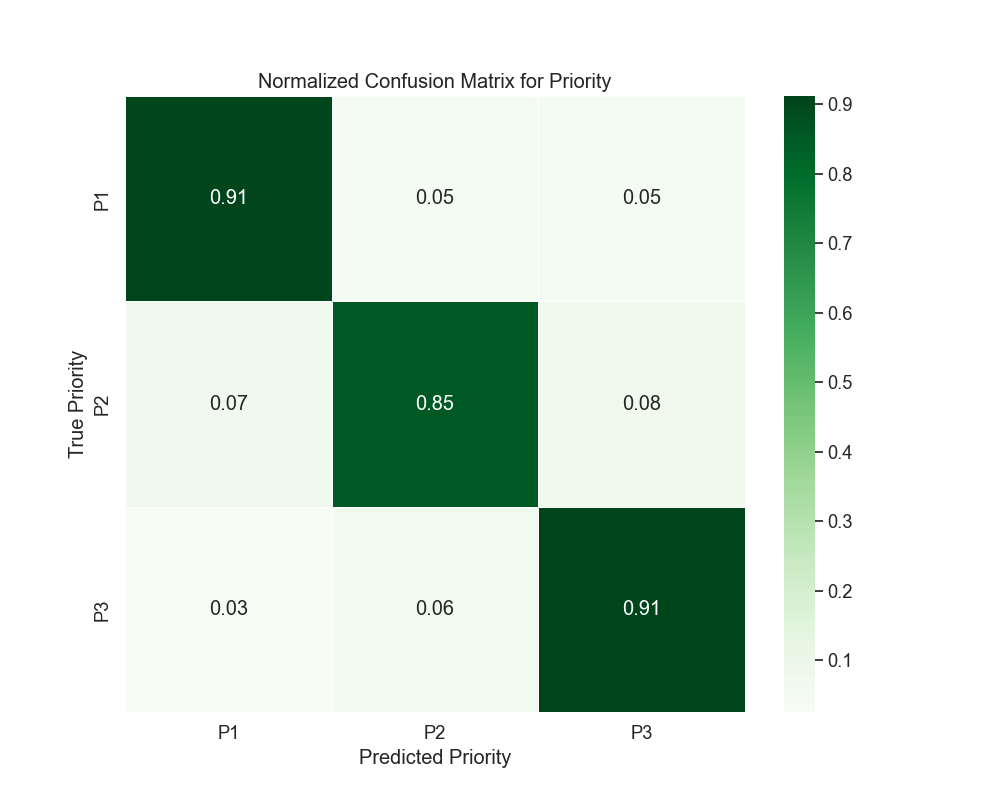
\includegraphics[width=\textwidth]{ch4/assets/v11_confusion_priority.png}
%         \caption{Confusion Matrix for Priority (Version 11)}
%         \label{fig:confusion_priority_v11}
%     \end{minipage}
%     \hfill
%     \begin{minipage}{0.49\textwidth}
%         \centering
%         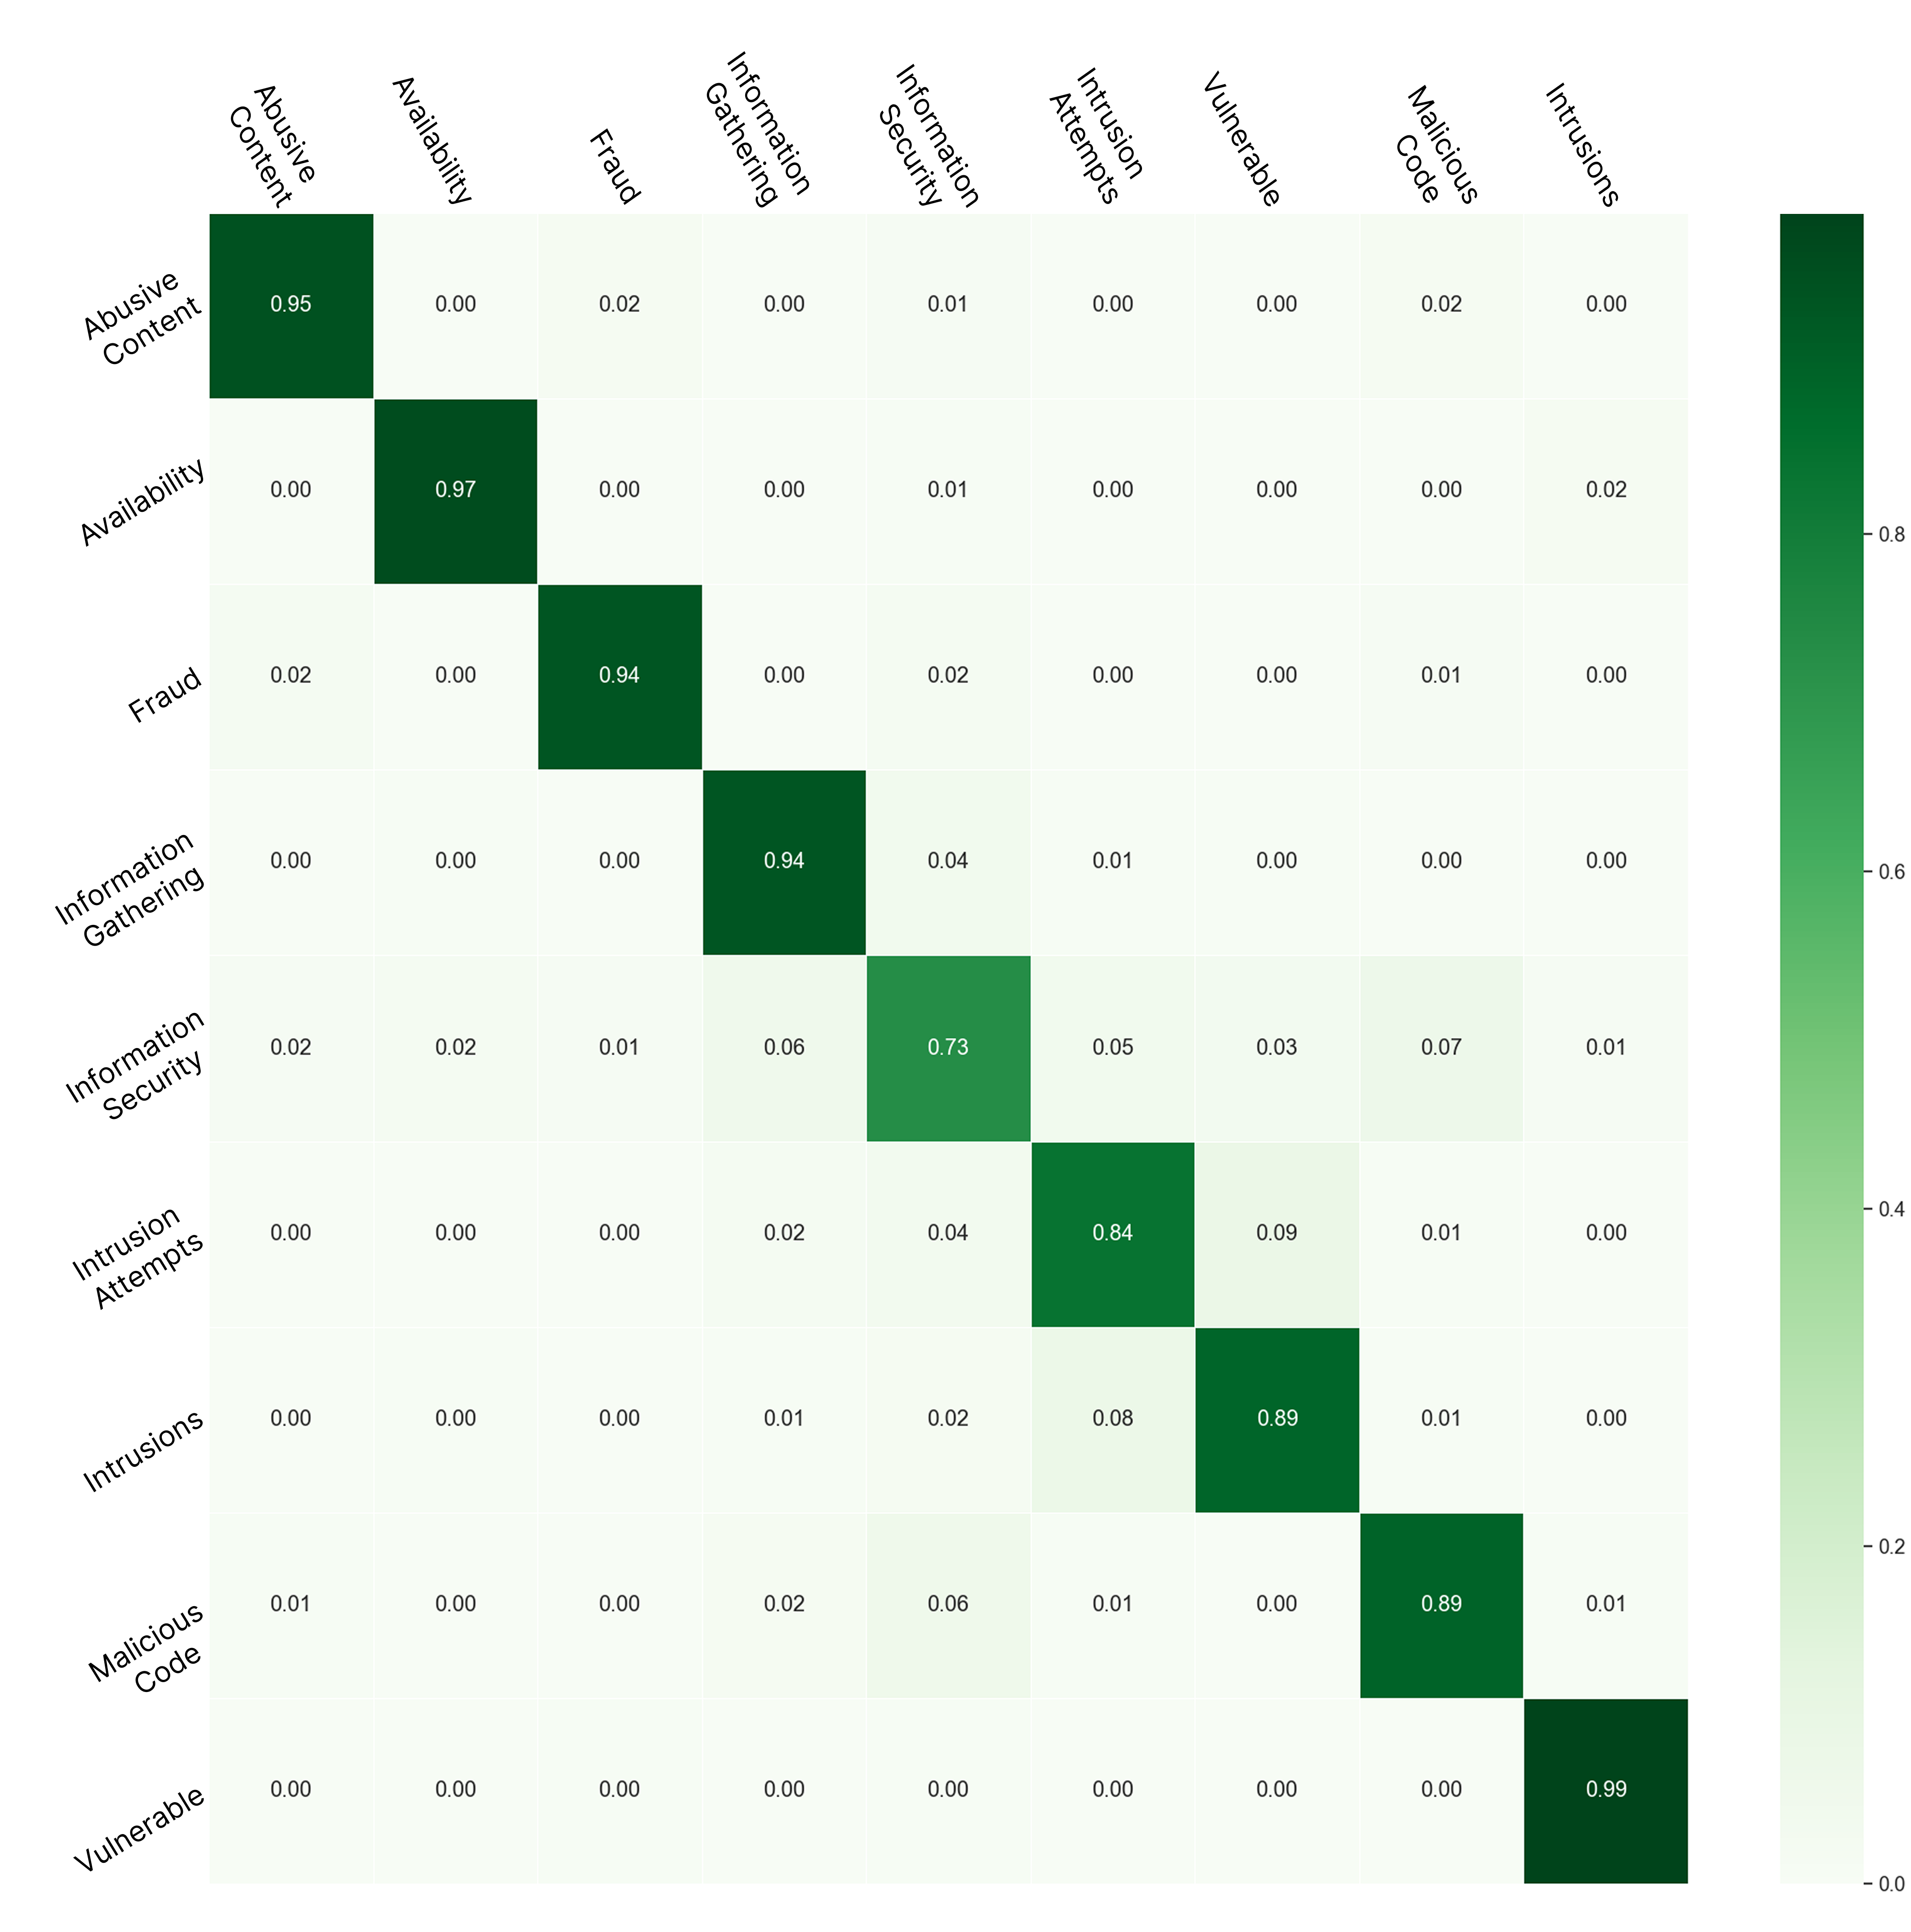
\includegraphics[width=\textwidth]{ch4/assets/v11_confusion_taxonomy.png}
%         \caption{Confusion Matrix for Taxonomy (Version 11)}
%         \label{fig:confusion_taxonomy_v11}
%     \end{minipage}
% \end{figure}

\begin{figure}[t!]
    \centering
    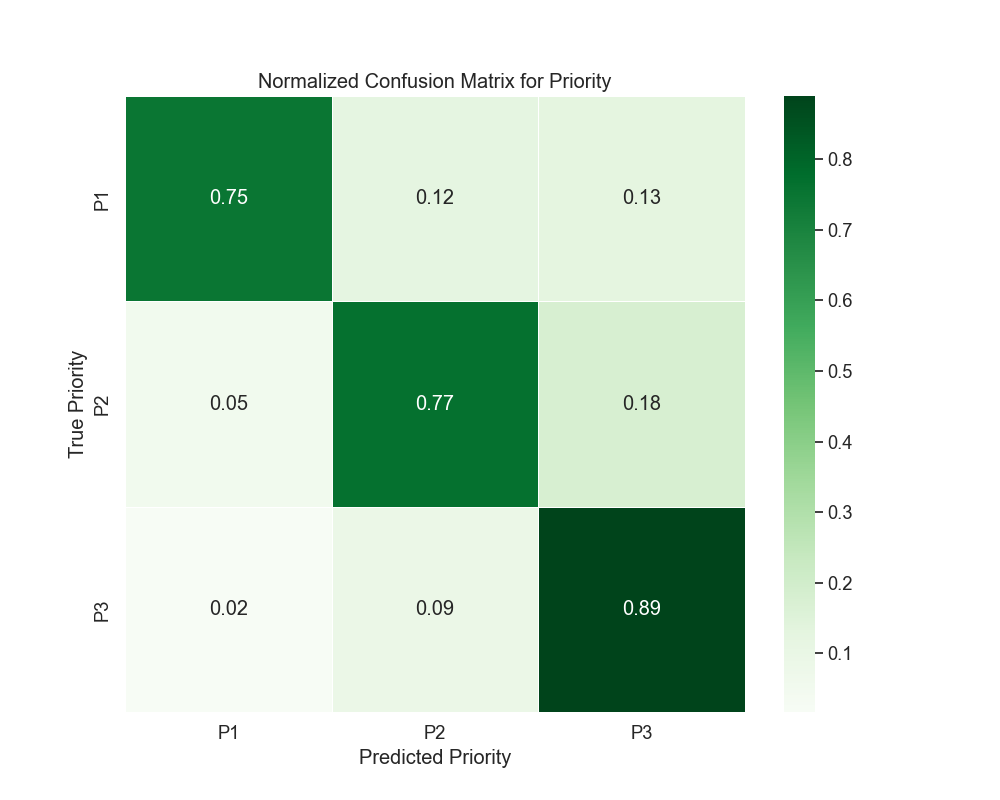
\includegraphics[width=0.8\textwidth]{ch4/assets/v1_confusion_priority.png}
    \caption{Confusion Matrix for Priority (Version 1)}
    \label{fig:confusion_priority_v1}
\end{figure}

\begin{figure}[b!]
    \centering
    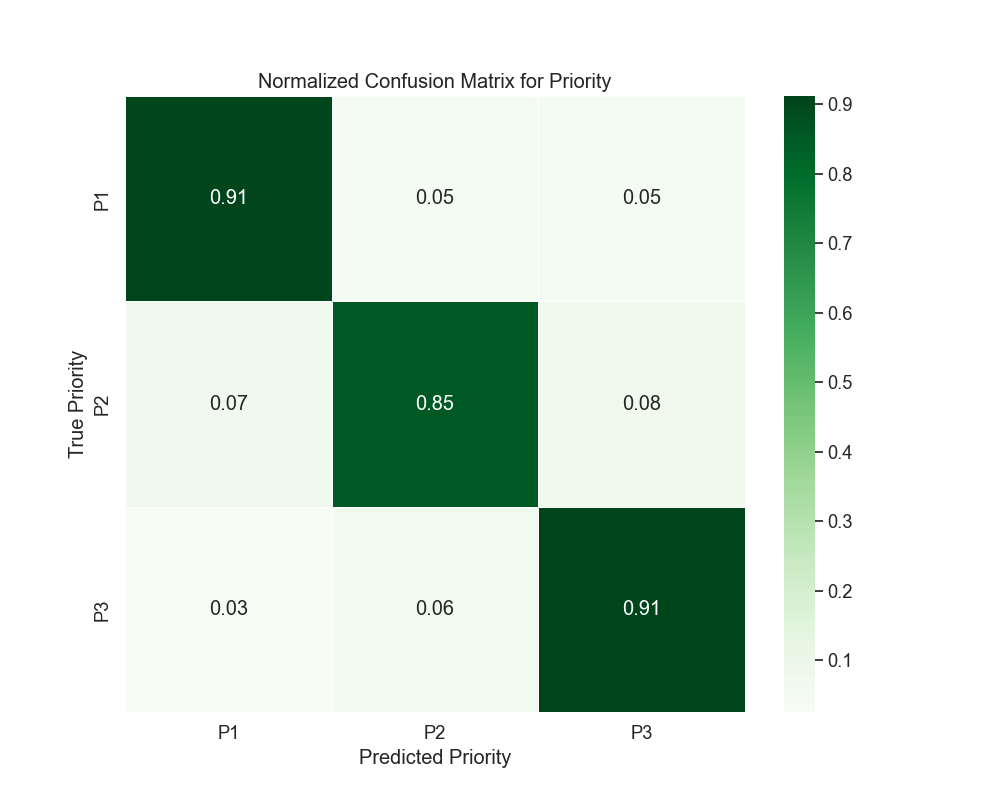
\includegraphics[width=0.8\textwidth]{ch4/assets/v11_confusion_priority.png}
    \caption{Confusion Matrix for Priority (Version 11)}
    \label{fig:confusion_priority_v11}
\end{figure}

\begin{figure}[t!]
    \centering
    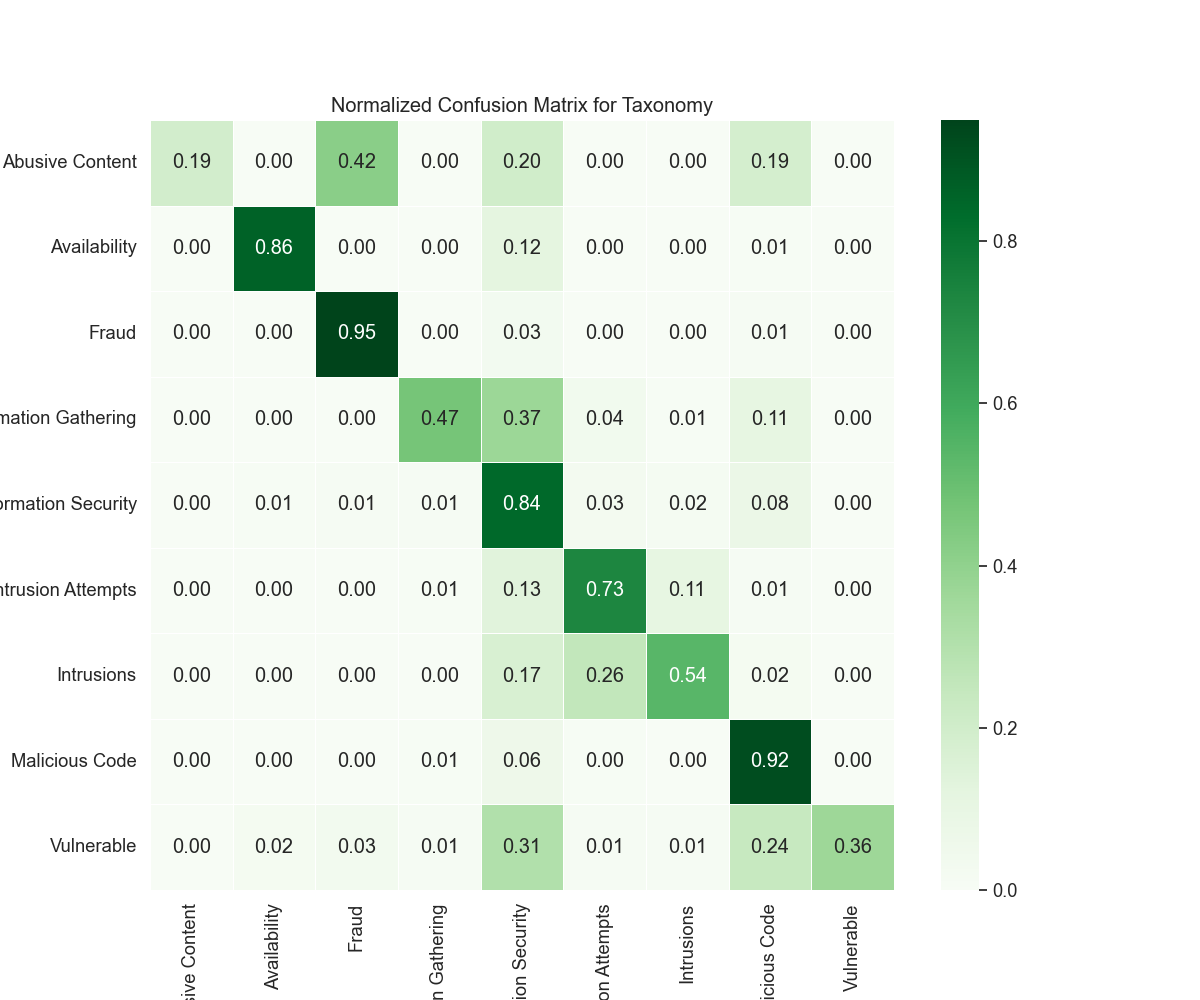
\includegraphics[width=0.8\textwidth]{ch4/assets/v1_confusion_taxonomy.png}
    \caption{Confusion Matrix for Taxonomy (Version 1)}
    \label{fig:confusion_taxonomy_v1}
\end{figure}

\begin{figure}[b!]
    \centering
    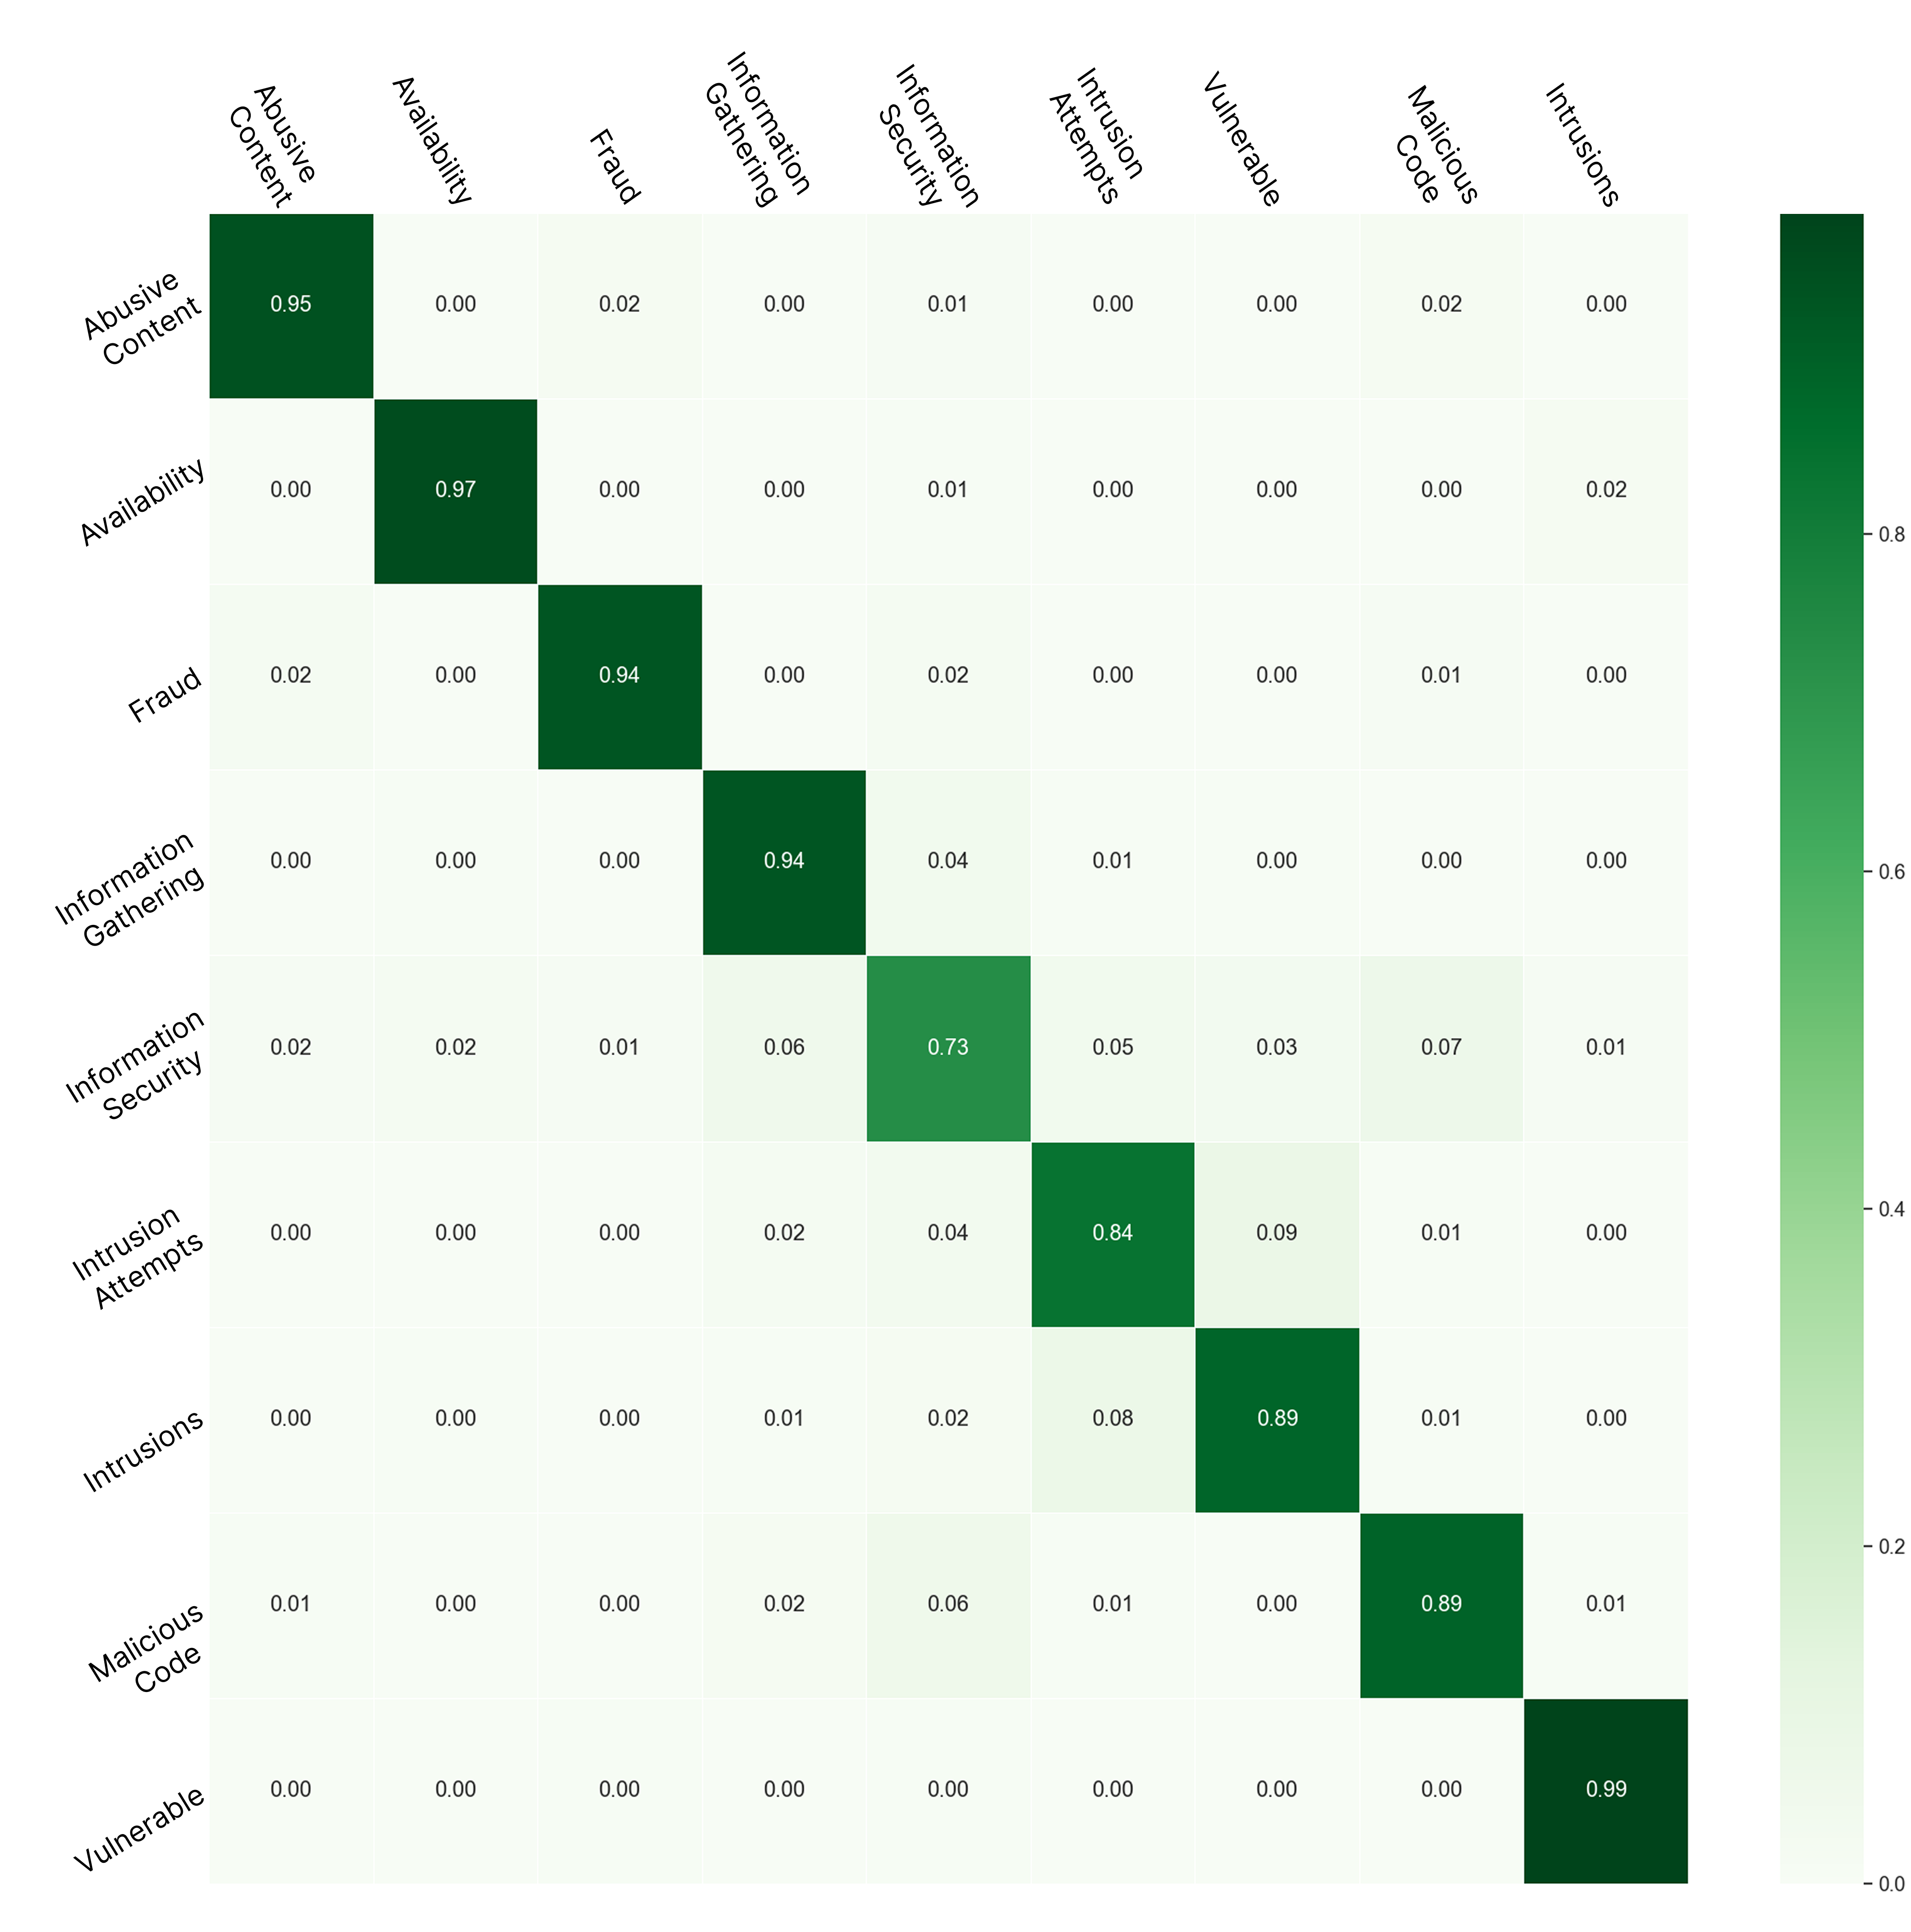
\includegraphics[width=0.8\textwidth]{ch4/assets/v11_confusion_taxonomy.png}
    \caption{Confusion Matrix for Taxonomy (Version 11)}
    \label{fig:confusion_taxonomy_v11}
\end{figure}

\clearpage 

The Table~\ref{tab:model_comparison} summarizes the key differences in the performance between Version 1 and Version 11 based on key metrics for both priority and taxonomy predictions.

% \captionsetup[table]{font=small} % Set the caption font size
% \scriptsize % Reduce the font size for the table content
\begin{longtable}{@{}P{3cm}P{3cm}P{4cm}P{4cm}@{}}
    \caption{Comparison of Model Performance: Version 1 vs. Version 11}
    \label{tab:model_comparison} \\
    \toprule
    \textbf{Metric} & \textbf{Version 1}  & \textbf{Version 11}  \\
    \midrule
    \endfirsthead

    \toprule
    \textbf{Metric} & \textbf{Version 1}  & \textbf{Version 11}  \\
    \midrule
    \endhead

    \bottomrule
    \endfoot

    \bottomrule
    \endlastfoot

    \textbf{Priority Accuracy} & 82\% & 90\% \\
    \vspace{0.2cm}
    \textbf{Taxonomy Accuracy} & 82\% & 90\% \\
    \vspace{0.2cm}
    \textbf{Recall for Low-Frequency Categories} & Moderate & High \\
    \vspace{0.2cm}
    \textbf{Recall for P2} & 70\% & 85\% \\
    \vspace{0.2cm}
    \textbf{Recall for P3} & 80\% & 91\% \\
\end{longtable}

When analyzing the table with the respective confusion matrixes, version 1 achieved 82\% accuracy for priority classification, which was a solid performance overall. 
However, the model faced challenges when distinguishing between P1 and P2 alerts. 
Many P2 alerts were misclassified as P1, likely due to their proximity in terms of severity, which the model struggled to differentiate in some instances.

While version 11 showed marked improvement with 90\% accuracy in priority classification. 
The recall for P2 and P3 categories improved significantly, with P2 recall increasing from 70\% in Version 1 to 85\% in Version 11. 
This improvement was achieved by better feature engineering and enhanced model tuning that allowed for more precise differentiation between priority levels. 
The increased recall for P3 (from 80\% to 91\%) demonstrated the model's improved capability to identify low-priority alerts without misclassifying them as high-priority.

In terms of taxonomies, version 1 achieved 82\% accuracy in taxonomy classification, which was satisfactory but left room for improvement in certain categories, particularly for minority classes like Vulnerable and Abusive Content. 
These categories were often misclassified due to the limited amount of training data and the imbalance in the dataset.

Version 11 saw a significant improvement, achieving 90\% accuracy in taxonomy classification. 
This improvement was particularly evident in the model's ability to handle low-frequency categories. For example, the recall for Vulnerable increased from 40\% in Version 1 to 75\% in Version 11, thanks to enhanced sampling strategies and better model adaptation. 
The Fraud and Intrusion Attempts categories also saw improvements in recall, confirming that the model's ability to classify common attack types remained strong while also improving its handling of less-represented categories.

\section{Live Testing Environment}

The live testing environment aims to simulate real-world deployment, where the models are evaluated based on their actual performance in the company's infrastructure. 
In this environment, both the RF and RL models are expected to be used. 
However, unlike the local environment where testing was done solely on the RF model, the live environment will also involve continuous training of the RL model. 
As feedback is gathered, the RL model is expected to improve its performance over time.

For the live testing, the application will not be evaluated separately on the RF and RL models but will instead use both models as part of an integrated system. 
During this phase, feedback from real-time predictions will be used to adjust and fine-tune the RL model's decisions. 
The expectation is that with time, the RL model will show improvements in its ability to predict priority and taxonomy, surpassing the performance of the initial RF model version.
